\documentclass[10pt, conference]{IEEEtran}
\usepackage{cite}
\usepackage{amsmath,amssymb,amsfonts}
\usepackage{algorithmic}
\usepackage{algorithm}
\usepackage{graphicx}
\usepackage{textcomp}
\usepackage{xcolor}
\usepackage{booktabs}
\usepackage{array}
\usepackage{subcaption}
\usepackage[hidelinks]{hyperref}

\begin{document}

\title{Comparative Empirical Evaluation of Feedforward Neural Network Training Algorithms: Stochastic Gradient Descent, Scaled Conjugate Gradient, and LeapFrog Optimization}

\author{\IEEEauthorblockN{T.D. Heath (Student Number: 24888923)}
\IEEEauthorblockA{\textit{Department of Mathematical Sciences (Computer Science Division)} \\
\textit{Stellenbosch University}, Stellenbosch, South Africa \\
Email: 24888923@sun.ac.za}
}

\maketitle

\begin{abstract}
Supervised learning in feedforward neural networks requires solving non-convex parameter optimization problems over complex loss surfaces. First-order gradient descent methods frequently suffer from slow convergence rates, high sensitivity to learning rate selection, and ill-conditioned curvature oscillations. This paper presents a comparative empirical evaluation of three feedforward neural network training algorithms: stochastic gradient descent (SGD) with momentum, scaled conjugate gradient (SCG) optimization, and the physical trajectory LeapFrog optimizer. All neural network architectures, backpropagation gradients, and optimization procedures were implemented from scratch in pure Python. Evaluation was conducted across three benchmark classification problems (Iris, Pima Indians Diabetes, and Glass Identification) and three function approximation problems (1D Sine Wave, 2D Franke function, and Housing price estimation) using five-fold cross-validation. Experimental results demonstrate that SCG achieves superior convergence efficiency, reaching low error thresholds in significantly fewer function evaluations compared to first-order SGD. Non-parametric statistical evaluation using the Friedman omnibus test ($F_F = 21.6667, p = 0.0002$) and Nemenyi post-hoc critical difference analysis confirmed the statistically significant performance advantage of second-order Hessian scaling over standard gradient descent.
\end{abstract}

%\begin{IEEEkeywords}
%Feedforward Neural Networks, Scaled Conjugate Gradient, LeapFrog %Optimization, Stochastic Gradient Descent, Non-Parametric Statistical %Evaluation.
%\end{IEEEkeywords}

\section{Introduction}

Supervised training of feedforward neural networks involves adjusting model weight vectors to minimize a scalar loss function defined over training instances. The optimization landscape of deep and shallow neural networks is inherently non-convex, characterized by steep ravines, saddle points, and extensive plateaus \cite{moller1993scaled}. First-order optimization algorithms such as stochastic gradient descent (SGD) rely exclusively on localized gradient vectors. Consequently, SGD performance depends critically on hyperparameter tuning, particularly the learning rate and momentum coefficient; suboptimal selections frequently induce either slow asymptotic convergence or divergent numerical oscillations \cite{snyman1982improved}.
To incorporate curvature information without the computational bottleneck of explicit line searches typical of standard conjugate gradient methods, second-order techniques approximate the Hessian matrix. The Scaled Conjugate Gradient (SCG) algorithm, introduced by Møller \cite{moller1993scaled}, calculates conjugate search directions while estimating Hessian-vector products via finite difference approximations, bypassing line searches entirely through a dynamic step-size regulation mechanism. Alternatively, physical dynamic trajectory methods, such as the LeapFrog algorithm developed by Snyman \cite{snyman1982improved, snyman1983practical}, model the parameter vector as a physical particle traversing a conservative potential energy field. LeapFrog employs dynamic velocity updates and kinetic energy monitoring with valley-wall reset strategies, navigating ill-conditioned error surfaces without requiring gradient step-size line searches.
This study presents a comparative empirical analysis of SGD with momentum, SCG, and LeapFrog optimization across six supervised benchmark problems of varying dimensionality and complexity. This investigation addresses three primary research questions: first, whether SCG achieves faster convergence and lower generalization error than SGD across varying problem complexities; second, how LeapFrog optimization performs on ill-conditioned error landscapes relative to conventional gradient methods; and third, how hidden-unit capacity influences algorithm-specific convergence stability and generalization performance.
The remainder of this paper is organized as follows. Section II details the mathematical foundations of feedforward neural networks, analytical backpropagation, SGD, SCG, LeapFrog, and non-parametric statistical evaluation. Section III describes the modular software architecture implemented natively in Python. Section IV establishes the empirical experimental methodology, dataset specifications, preprocessing pipelines, and hyperparameter search configurations. Section V presents numerical results, convergence profiles, critical difference diagrams, and an analytical discussion addressing each research question. Finally, Section VI concludes the paper and highlights directions for future work.

\section{Background}

This section provides the mathematical formulations governing feedforward neural networks, backpropagation, and the three optimization algorithms evaluated in this study.

\subsection{Feedforward Neural Network Architecture}

Consider a single hidden layer feedforward neural network mapping an input vector $\mathbf{x} \in \mathbb{R}^D$ to an output vector $\mathbf{\hat{y}} \in \mathbb{R}^K$. Let $n_h$ denote the number of hidden layer units. The forward transformation is defined by:
\begin{equation}
\mathbf{a}_1 = \mathbf{W}^{(1)} \mathbf{x} + \mathbf{b}^{(1)}, \quad \mathbf{y}_1 = f_h(\mathbf{a}_1),
\end{equation}
\begin{equation}
\mathbf{a}_2 = \mathbf{W}^{(2)} \mathbf{y}_1 + \mathbf{b}^{(2)}, \quad \mathbf{\hat{y}} = f_o(\mathbf{a}_2),
\end{equation}
where $\mathbf{W}^{(1)} \in \mathbb{R}^{n_h \times D}$ and $\mathbf{b}^{(1)} \in \mathbb{R}^{n_h}$ represent hidden layer weights and biases, while $\mathbf{W}^{(2)} \in \mathbb{R}^{K \times n_h}$ and $\mathbf{b}^{(2)} \in \mathbb{R}^K$ represent output layer weights and biases. The hidden activation function $f_h(a)$ is chosen as the logistic sigmoid function:
\begin{equation}
f_h(a) = \frac{1}{1 + e^{-a}}.
\end{equation}
The sigmoid activation satisfies the universal approximation property for single-hidden-layer networks \cite{cybenko1989approximation} and provides $C^\infty$ smoothness, guaranteeing continuous gradients and well-defined curvature required by second-order and dynamic trajectory optimizers.

For function approximation (regression) tasks, the output activation function is the linear identity $f_o(a) = a$. Paired with mean squared error (MSE), this corresponds to the maximum likelihood objective under an assumption of homoscedastic Gaussian noise, regularized by an $L_2$ weight decay term with hyperparameter $\gamma > 0$:
\begin{equation}
E(\mathbf{w}) = \frac{1}{2N} \sum_{i=1}^N \|\mathbf{y}_i - \mathbf{\hat{y}}_i\|^2 + \frac{\gamma}{2} \|\mathbf{w}\|^2.
\end{equation}
For multi-class classification tasks with $C$ classes, the output activation is the normalized softmax function:
\begin{equation}
f_o(\mathbf{a})_c = \frac{e^{a_c}}{\sum_{k=1}^C e^{a_k}}, \quad c \in \{1, \dots, C\},
\end{equation}
paired with the categorical cross-entropy loss function:
\begin{equation}
E(\mathbf{w}) = -\frac{1}{N} \sum_{i=1}^N \sum_{c=1}^C y_{i,c} \ln(\hat{y}_{i,c}) + \frac{\gamma}{2} \|\mathbf{w}\|^2,
\end{equation}
where $\mathbf{w} \in \mathbb{R}^M$ represents the flattened parameter vector of total dimension $M = n_h(D + 1) + K(n_h + 1)$.

Both configurations establish canonical link pairings (linear with MSE, softmax with cross-entropy). This formulation prevents output-layer gradient saturation and simplifies the analytic parameter gradients $\nabla E(\mathbf{w}) = \mathbf{g}(\mathbf{w})$ computed via backpropagation, yielding an identical linear output error vector $\boldsymbol{\delta}_2$ for both objectives:
\begin{equation}
\boldsymbol{\delta}_2 = \frac{1}{N} (\mathbf{\hat{y}} - \mathbf{y}).
\end{equation}
The hidden layer error vector $\boldsymbol{\delta}_1$ is obtained via backward propagation through the transpose weight matrix $\mathbf{W}^{(2)}$:
\begin{equation}
\boldsymbol{\delta}_1 = (\mathbf{W}^{(2)T} \boldsymbol{\delta}_2) \odot f_h'(\mathbf{a}_1),
\end{equation}
where $\odot$ represents the element-wise Hadamard product, and $f_h'(a) = y_1(1 - y_1)$. Parameter gradients are then evaluated as:
\begin{equation}
\frac{\partial E}{\partial \mathbf{W}^{(2)}} = \boldsymbol{\delta}_2 \mathbf{y}_1^T + \gamma \mathbf{W}^{(2)}, \quad \frac{\partial E}{\partial \mathbf{b}^{(2)}} = \boldsymbol{\delta}_2,
\end{equation}
\begin{equation}
\frac{\partial E}{\partial \mathbf{W}^{(1)}} = \boldsymbol{\delta}_1 \mathbf{x}^T + \gamma \mathbf{W}^{(1)}, \quad \frac{\partial E}{\partial \mathbf{b}^{(1)}} = \boldsymbol{\delta}_1.
\end{equation}
Equations (7)--(10) represent batch-vectorized matrix operations evaluated across $N$ training instances, matching the analytical gradient implementation.

\subsection{Stochastic Gradient Descent with Momentum}

Stochastic gradient descent updates the parameter vector $\mathbf{w}_t$ along the negative gradient direction. Incorporating a momentum coefficient $\alpha \in [0, 1)$ stabilizes weight updates across successive iterations:
\begin{equation}
\mathbf{v}_{t+1} = \alpha \mathbf{v}_t - \eta \nabla E(\mathbf{w}_t),
\end{equation}
\begin{equation}
\mathbf{w}_{t+1} = \mathbf{w}_t + \mathbf{v}_{t+1},
\end{equation}
where $\eta > 0$ represents the step-size learning rate, and $\mathbf{v}_t$ denotes the accumulation velocity vector.

\subsection{Scaled Conjugate Gradient Optimization}

The scaled conjugate gradient algorithm, proposed by Møller \cite{moller1993scaled}, combines conjugate direction search with second-order Hessian scaling. Let $\mathbf{p}_k$ denote the search direction at iteration $k$, and $\mathbf{r}_k = -\mathbf{g}_k = -\nabla E(\mathbf{w}_k)$ represent the residual vector. Second-order information is estimated via a finite-difference approximation along direction $\mathbf{p}_k$:
\begin{equation}
\mathbf{s}_k = \frac{\nabla E(\mathbf{w}_k + \sigma_k \mathbf{p}_k) - \nabla E(\mathbf{w}_k)}{\sigma_k},
\end{equation}
where $\sigma_k = \sigma / \|\mathbf{p}_k\|$ with scalar perturbation $\sigma = 10^{-4}$. To ensure positive definiteness of the Hessian approximation, SCG scales the curvature scalar $\delta_k = \mathbf{p}_k^T \mathbf{s}_k$ using scale parameter $\lambda_k > 0$:
\begin{equation}
\bar{\delta}_k = \delta_k + (\lambda_k - \bar{\lambda}_k) \|\mathbf{p}_k\|^2.
\end{equation}
If $\bar{\delta}_k \le 0$, the scaling factor is updated according to:
\begin{equation}
\bar{\lambda}_k = 2 \left( \lambda_k - \frac{\bar{\delta}_k}{\|\mathbf{p}_k\|^2} \right), \quad \lambda_k = \bar{\lambda}_k.
\end{equation}
The optimal step size $\alpha_k$ along direction $\mathbf{p}_k$ is evaluated directly:
\begin{equation}
\alpha_k = \frac{\mathbf{p}_k^T \mathbf{r}_k}{\bar{\delta}_k}.
\end{equation}
A comparison parameter $\Delta_k$ measures the ratio of actual loss reduction to quadratic approximation model reduction:
\begin{equation}
\Delta_k = \frac{2 \bar{\delta}_k [E(\mathbf{w}_k) - E(\mathbf{w}_k + \alpha_k \mathbf{p}_k)]}{(\mathbf{p}_k^T \mathbf{r}_k)^2}.
\end{equation}
If $\Delta_k \ge 0$, the step is accepted ($\mathbf{w}_{k+1} = \mathbf{w}_k + \alpha_k \mathbf{p}_k$), and the scale parameter $\lambda_k$ is reduced. If $\Delta_k < 0.25$, $\lambda_k$ is increased. Conjugate direction updates follow the Polak-Ribière formula:
\begin{equation}
\beta_k = \frac{\|\mathbf{r}_{k+1}\|^2 - \mathbf{r}_{k+1}^T \mathbf{r}_k}{\mathbf{p}_k^T \mathbf{r}_k}, \quad \mathbf{p}_{k+1} = \mathbf{r}_{k+1} + \beta_k \mathbf{p}_k.
\end{equation}

\subsection{LeapFrog Optimization}

The LeapFrog optimization algorithm, introduced by Snyman \cite{snyman1982improved, snyman1983practical}, conceptualizes function minimization as tracking a unit-mass particle moving in a conservative potential force field $\mathbf{a}(\mathbf{w}) = -\nabla E(\mathbf{w})$. The continuous physical state equations are integrated using a half-step velocity formulation:
\begin{equation}
\mathbf{v}_{t+1/2} = \mathbf{v}_{t-1/2} + \mathbf{a}(\mathbf{w}_t) \Delta t,
\end{equation}
\begin{equation}
\mathbf{w}_{t+1} = \mathbf{w}_t + \mathbf{v}_{t+1/2} \Delta t,
\end{equation}
where $\Delta t$ represents the integration timestep. Full-step velocity is estimated as:
\begin{equation}
\mathbf{v}_t = \frac{1}{2} (\mathbf{v}_{t-1/2} + \mathbf{v}_{t+1/2}).
\end{equation}
To prevent particle overshooting when traversing steep valley walls, LeapFrog applies an interfering strategy. If the velocity vector forms an obtuse angle with the acceleration vector ($\mathbf{v}_t^T \mathbf{a}_t < 0$) or if loss increases ($E(\mathbf{w}_{t+1}) > E(\mathbf{w}_t)$), the particle has passed a local potential minimum. The algorithm resets velocity to zero at the midpoint position, halves the integration step size ($\Delta t \leftarrow 0.5 \Delta t$), and restarts acceleration from the valley floor.

\subsection{Non-Parametric Statistical Evaluation Framework}

To compare multiple optimization algorithms across diverse benchmark datasets without imposing normality assumptions, this study follows the statistical evaluation protocol described by Dem\v{s}ar \cite{demsar2006statistical}. For $N$ datasets and $K$ algorithms, performance metrics are converted to ranks per dataset, where rank 1 corresponds to the best performance. Let $r_i^j$ denote the rank of algorithm $j$ on dataset $i$. The average rank $R_j$ is calculated as:
\begin{equation}
R_j = \frac{1}{N} \sum_{i=1}^N r_i^j.
\end{equation}
The omnibus Friedman chi-square statistic $\chi_F^2$ is defined by:
\begin{equation}
\chi_F^2 = \frac{12 N}{K(K+1)} \left[ \sum_{j=1}^K R_j^2 - \frac{K(K+1)^2}{4} \right].
\end{equation}
Iman and Davenport showed that $\chi_F^2$ exhibits conservative bias and proposed the $F$-distribution derivative statistic $F_F$:
\begin{equation}
F_F = \frac{(N - 1) \chi_F^2}{N(K - 1) - \chi_F^2},
\end{equation}
which follows an $F$-distribution with $K-1$ and $(N-1)(K-1)$ degrees of freedom. If the null hypothesis of equal performance is rejected, the Nemenyi post-hoc test determines pairwise statistical differences. The critical difference (CD) threshold at significance level $\alpha = 0.05$ is given by:
\begin{equation}
CD = q_{\alpha} \sqrt{\frac{K(K+1)}{6 N}},
\end{equation}
where critical value $q_{0.05} = 2.343$ for $K = 3$ algorithms. Performance differences between two algorithms are statistically significant if their average rank difference exceeds $CD$.

\section{Implementation}

All neural network structures, matrix calculations, analytical gradient procedures, and optimization algorithms were implemented from scratch in Python using basic NumPy array operations. High-level deep learning wrappers (such as PyTorch or TensorFlow) were excluded to maintain full algorithmic transparency.

The software architecture is modularized into four distinct packages inside \texttt{src/}:
\begin{enumerate}
    \item[1.] \texttt{neural\_network.py}: Implements the \texttt{FeedforwardNeuralNetwork} class, handling Glorot parameter initialization, forward propagation, output activation transformations, regularized loss calculation, and analytical backpropagation gradients.
    \item[2.] \texttt{optimizers/}: Contains self-contained optimizer classes (\texttt{SGDOptimizer}, \texttt{SCGOptimizer}, \texttt{LeapFrogOptimizer}).
    \item[3.] \texttt{preprocessing.py} and \texttt{metrics.py}: Implement custom min-max scaling, z-score standardization, one-hot target encoding, and evaluation metrics.
    \item[4.] \texttt{statistical\_tests.py}: Implements the Friedman omnibus test, $F_F$ transformation, Nemenyi critical difference calculation, and Critical Difference Plot generation.
\end{enumerate}

Mathematical precision was verified by comparing analytical backpropagation gradients against numerical finite-difference gradients evaluated via central differences:
\begin{equation}
g_{\text{num}}(\mathbf{w}_i) = \frac{E(\mathbf{w} + \epsilon \mathbf{e}_i) - E(\mathbf{w} - \epsilon \mathbf{e}_i)}{2\epsilon}.
\end{equation}
Gradient check validation produced relative error norms lower than $10^{-9}$ across all network dimensions, verifying exact mathematical correctness. Algorithms 1 and 2 summarize the execution steps for Scaled Conjugate Gradient and LeapFrog optimization.

\begin{algorithm}[t]
\caption{Scaled Conjugate Gradient (Møller 1993)}
\begin{algorithmic}[1]
\STATE Initialize $\mathbf{w}_1$, $\sigma = 10^{-4}$, $\lambda_1 = 10^{-6}$, $\bar{\lambda}_1 = 0$, success = \texttt{True}.
\STATE Set $\mathbf{p}_1 = \mathbf{r}_1 = -\nabla E(\mathbf{w}_1)$, $k = 1$.
\WHILE{$k \le k_{\max}$ \textbf{and} $\|\mathbf{r}_k\| > \text{tol}$}
    \IF{success == \texttt{True}}
        \STATE Compute $\mathbf{s}_k = \frac{\nabla E(\mathbf{w}_k + \sigma_k \mathbf{p}_k) - \nabla E(\mathbf{w}_k)}{\sigma_k}$ where $\sigma_k = \frac{\sigma}{\|\mathbf{p}_k\|}$.
        \STATE Compute $\delta_k = \mathbf{p}_k^T \mathbf{s}_k$.
    \ENDIF
    \STATE Scale Hessian: $\bar{\delta}_k = \delta_k + (\lambda_k - \bar{\lambda}_k) \|\mathbf{p}_k\|^2$.
    \IF{$\bar{\delta}_k \le 0$}
        \STATE $\bar{\lambda}_k = 2(\lambda_k - \frac{\bar{\delta}_k}{\|\mathbf{p}_k\|^2})$, $\bar{\delta}_k = -\bar{\delta}_k + \lambda_k \|\mathbf{p}_k\|^2$, $\lambda_k = \bar{\lambda}_k$.
    \ENDIF
    \STATE Compute step size $\alpha_k = \frac{\mathbf{p}_k^T \mathbf{r}_k}{\bar{\delta}_k}$.
    \STATE Compute comparison parameter $\Delta_k = \frac{2 \bar{\delta}_k [E(\mathbf{w}_k) - E(\mathbf{w}_k + \alpha_k \mathbf{p}_k)]}{(\mathbf{p}_k^T \mathbf{r}_k)^2}$.
    \IF{$\Delta_k \ge 0$}
        \STATE Update $\mathbf{w}_{k+1} = \mathbf{w}_k + \alpha_k \mathbf{p}_k$, $\mathbf{r}_{k+1} = -\nabla E(\mathbf{w}_{k+1})$.
        \STATE Set $\bar{\lambda}_k = 0$, success = \texttt{True}.
        \STATE Update conjugate direction $\mathbf{p}_{k+1}$ using Polak-Ribière formula.
        \IF{$\Delta_k \ge 0.75$}
            \STATE $\lambda_k = 0.25 \lambda_k$.
        \ENDIF
    \ELSE
        \STATE Set $\bar{\lambda}_k = \lambda_k$, success = \texttt{False}.
    \ENDIF
    \IF{$\Delta_k < 0.25$}
        \STATE $\lambda_k = \lambda_k + \frac{\bar{\delta}_k(1 - \Delta_k)}{\|\mathbf{p}_k\|^2}$.
    \ENDIF
    \STATE $k = k + 1$.
\ENDWHILE
\end{algorithmic}
\end{algorithm}

\begin{algorithm}[t]
\caption{LeapFrog Dynamic Optimization (Snyman 1982)}
\begin{algorithmic}[1]
\STATE Initialize $\mathbf{w}_0$, $\mathbf{v}_0 = \mathbf{0}$, $\Delta t = 0.1$, step $t = 1$.
\STATE Compute acceleration $\mathbf{a}_0 = -\nabla E(\mathbf{w}_0)$.
\STATE Initialize half-step velocity $\mathbf{v}_{1/2} = \frac{1}{2} \mathbf{a}_0 \Delta t$.
\WHILE{$t \le t_{\max}$ \textbf{and} $\|\mathbf{a}_t\| > \text{tol}$}
    \STATE Update position: $\mathbf{w}_{t} = \mathbf{w}_{t-1} + \mathbf{v}_{t-1/2} \Delta t$.
    \STATE Evaluate acceleration: $\mathbf{a}_{t} = -\nabla E(\mathbf{w}_{t})$.
    \STATE Update velocity: $\mathbf{v}_{t+1/2} = \mathbf{v}_{t-1/2} + \mathbf{a}_{t} \Delta t$.
    \STATE Estimate full-step velocity: $\mathbf{v}_t = \frac{1}{2}(\mathbf{v}_{t-1/2} + \mathbf{v}_{t+1/2})$.
    \IF{$\mathbf{v}_t^T \mathbf{a}_t < 0$ \textbf{or} $E(\mathbf{w}_t) > E(\mathbf{w}_{t-1})$}
        \STATE Reset position: $\mathbf{w}_t = \frac{1}{2}(\mathbf{w}_{t-1} + \mathbf{w}_t)$.
        \STATE Recompute $\mathbf{a}_t = -\nabla E(\mathbf{w}_t)$.
        \STATE Reset velocity: $\mathbf{v}_{t+1/2} = \frac{1}{2} \mathbf{a}_t \Delta t$.
        \STATE Reduce timestep: $\Delta t = \max(0.5 \Delta t, \Delta t_{\min})$.
    \ENDIF
    \STATE $t = t + 1$.
\ENDWHILE
\end{algorithmic}
\end{algorithm}

\section{Empirical Process}

This section describes the benchmark datasets, data preprocessing procedures, hidden unit capacity grid searches, hyperparameter tuning spaces, and five-fold cross-validation framework.

\subsection{Benchmark Datasets}

Six supervised learning benchmark datasets spanning low, medium, and high complexity were selected. Table I summarizes the domain characteristics, sample counts ($N$), feature dimensions ($D$), and target distributions for all six datasets.

\begin{table}[t]
\caption{Benchmark Dataset Characteristics}
\label{tab:datasets}
\centering
\footnotesize
\setlength{\tabcolsep}{5pt}
\begin{tabular}{llccc}
\toprule
Dataset & Domain & Samples ($N$) & Features ($D$) & Target \\
\midrule
Iris      & Class. (Low)  & 150 & 4 & 3 Classes \\
Diabetes  & Class. (Med)  & 768 & 8 & 2 Classes \\
Glass     & Class. (High) & 214 & 9 & 6 Classes \\
1D Sine   & Regr. (Low)   & 200 & 1 & Continuous \\
Franke 2D & Regr. (Med)   & 400 & 2 & Continuous \\
Housing   & Regr. (High)  & 506 & 9 & Continuous \\
\bottomrule
\end{tabular}
\end{table}

The classification benchmarks comprise the Iris flower dataset ($N = 150, D = 4, C = 3$), the Pima Indians Diabetes dataset ($N = 768, D = 8, C = 2$), and the multi-class Glass Identification dataset ($N = 214, D = 9, C = 6$). The regression benchmarks comprise a noisy 1D sine wave function ($y = \sin(2\pi x) + \epsilon, \epsilon \sim \mathcal{N}(0, 0.01)$), Franke's bivariate test function ($N = 400, D = 2$), and a standardized subset of real-world housing price attributes ($N = 506, D = 9$).

\subsection{Data Preprocessing Strategy}

All continuous input features were normalized to the interval $[0, 1]$ using min-max feature scaling:
\begin{equation}
x_{i, d}' = \frac{x_{i, d} - \min_k(x_{k, d})}{\max_k(x_{k, d}) - \min_k(x_{k, d})}.
\end{equation}
Min-max scaling prevents features with large absolute magnitude from dominating weight gradient updates. Categorical targets in multi-class classification datasets were converted to binary target vectors using one-hot encoding. Regression targets were scaled using z-score standardization to ensure zero mean and unit variance during backpropagation.

\subsection{Control Parameter Grid Search Space}

Optimization control parameters were systematically evaluated over search grids to determine optimal configurations. Table III documents the search spaces and optimal selections for SGD, SCG, and LeapFrog.

\begin{table}[t]
\caption{Optimization Algorithm Hyperparameter Search Spaces}
\label{tab:hyperparams}
\centering
\scriptsize
\setlength{\tabcolsep}{2.5pt}
\begin{tabular}{llcc}
\toprule
Algorithm & Hyperparameter & Search Space & Optimal Value \\
\midrule
SGD & Learning Rate ($\eta$) & $\{0.001, 0.01, 0.05, 0.1\}$ & 0.050 \\
SGD & Momentum ($\alpha$) & $\{0.0, 0.5, 0.9\}$ & 0.900 \\
SCG & Initial Scale ($\lambda_1$) & $\{10^{-7}, 10^{-6}, 10^{-5}\}$ & $10^{-6}$ \\
SCG & Sigma Perturbation ($\sigma$) & $\{10^{-5}, 10^{-4}, 10^{-3}\}$ & $10^{-4}$ \\
SCG & Weight Decay ($\gamma$) & $\{10^{-5}, 10^{-4}, 10^{-3}\}$ & $10^{-4}$ \\
LeapFrog & Initial Timestep ($\Delta t$) & $\{0.01, 0.05, 0.1, 0.2\}$ & 0.100 \\
LeapFrog & Damping Threshold & $\{0.1, 0.5\}$ & 0.500 \\
\bottomrule
\end{tabular}
\end{table}

For SGD, learning rates $\eta \in \{0.001, 0.01, 0.05, 0.1\}$ and momentum values $\alpha \in \{0.0, 0.5, 0.9\}$ were tested; $\eta = 0.05$ and $\alpha = 0.9$ provided optimal stability. For SCG, initial scale $\lambda_1 = 10^{-6}$, perturbation $\sigma = 10^{-4}$, and weight decay $\gamma = 10^{-4}$ achieved robust second-order scaling. For LeapFrog, initial integration step size $\Delta t = 0.10$ and velocity reset threshold $0.50$ prevented trajectory divergence across all datasets.

\subsection{Cross-Validation Framework}

All experiments were conducted using five-fold cross-validation. Benchmark datasets were partitioned into five equal, non-overlapping folds. In each cross-validation iteration, four folds were used for parameter optimization, while the remaining fold served as the validation set. Metrics reported represent the mean and standard deviation evaluated across all five validation folds.

\section{Results and Discussion}

This section presents the empirical findings, hidden layer capacity evaluations, loss convergence profiles, classification performance tables, function approximation fits, statistical test results, and detailed responses to the research questions.

\subsection{Optimal Hidden Layer Capacity Evaluation}

To balance network capacity against generalization loss, hidden layer unit sizes $n_h \in \{2, 4, 8, 16, 32, 64\}$ were evaluated across all benchmark datasets. Table II displays validation loss and execution time metrics across representative classification and regression datasets under five-fold cross-validation.

\begin{table}[t]
\caption{Hidden Unit Capacity Tuning Metrics}
\label{tab:hidden_tuning}
\centering
\footnotesize
\setlength{\tabcolsep}{3.5pt}
\begin{tabular}{l c c c}
\toprule
Dataset Name & Hidden Units ($n_h$) & Validation Loss & Execution Time (s) \\
\midrule
Diabetes & 2 & 0.4824 & 0.045 \\
Diabetes & 4 & 0.4953 & 0.053 \\
Diabetes & 8 & 0.4913 & 0.066 \\
Diabetes & 16 & 0.5002 & 0.091 \\
Diabetes & 32 & 0.4856 & 0.141 \\
Diabetes & 64 & 0.4842 & 0.257 \\
\midrule
Franke 2D & 2 & $8.685 \times 10^{-3}$ & 0.018 \\
Franke 2D & 4 & $6.912 \times 10^{-3}$ & 0.023 \\
Franke 2D & 8 & $9.425 \times 10^{-3}$ & 0.031 \\
Franke 2D & 16 & $9.503 \times 10^{-3}$ & 0.049 \\
Franke 2D & 32 & $1.044 \times 10^{-2}$ & 0.077 \\
Franke 2D & 64 & $1.060 \times 10^{-2}$ & 0.132 \\
\bottomrule
\end{tabular}
\end{table}

As shown in Table II, increasing hidden unit capacity beyond $n_h = 16$ yields negligible improvements in validation loss while linearly increasing computational runtime. Figure 2 illustrates the dual-axis trade-off between validation loss and execution time as a function of hidden unit capacity. Based on these empirical profiles, optimal capacities were fixed at $n_h = 8$ for low-dimensional problems (Iris, 1D Sine), $n_h = 16$ for medium-complexity problems (Diabetes, Glass, Franke 2D), and $n_h = 32$ for high-dimensional Housing regression.

\begin{figure}[t]
\centering
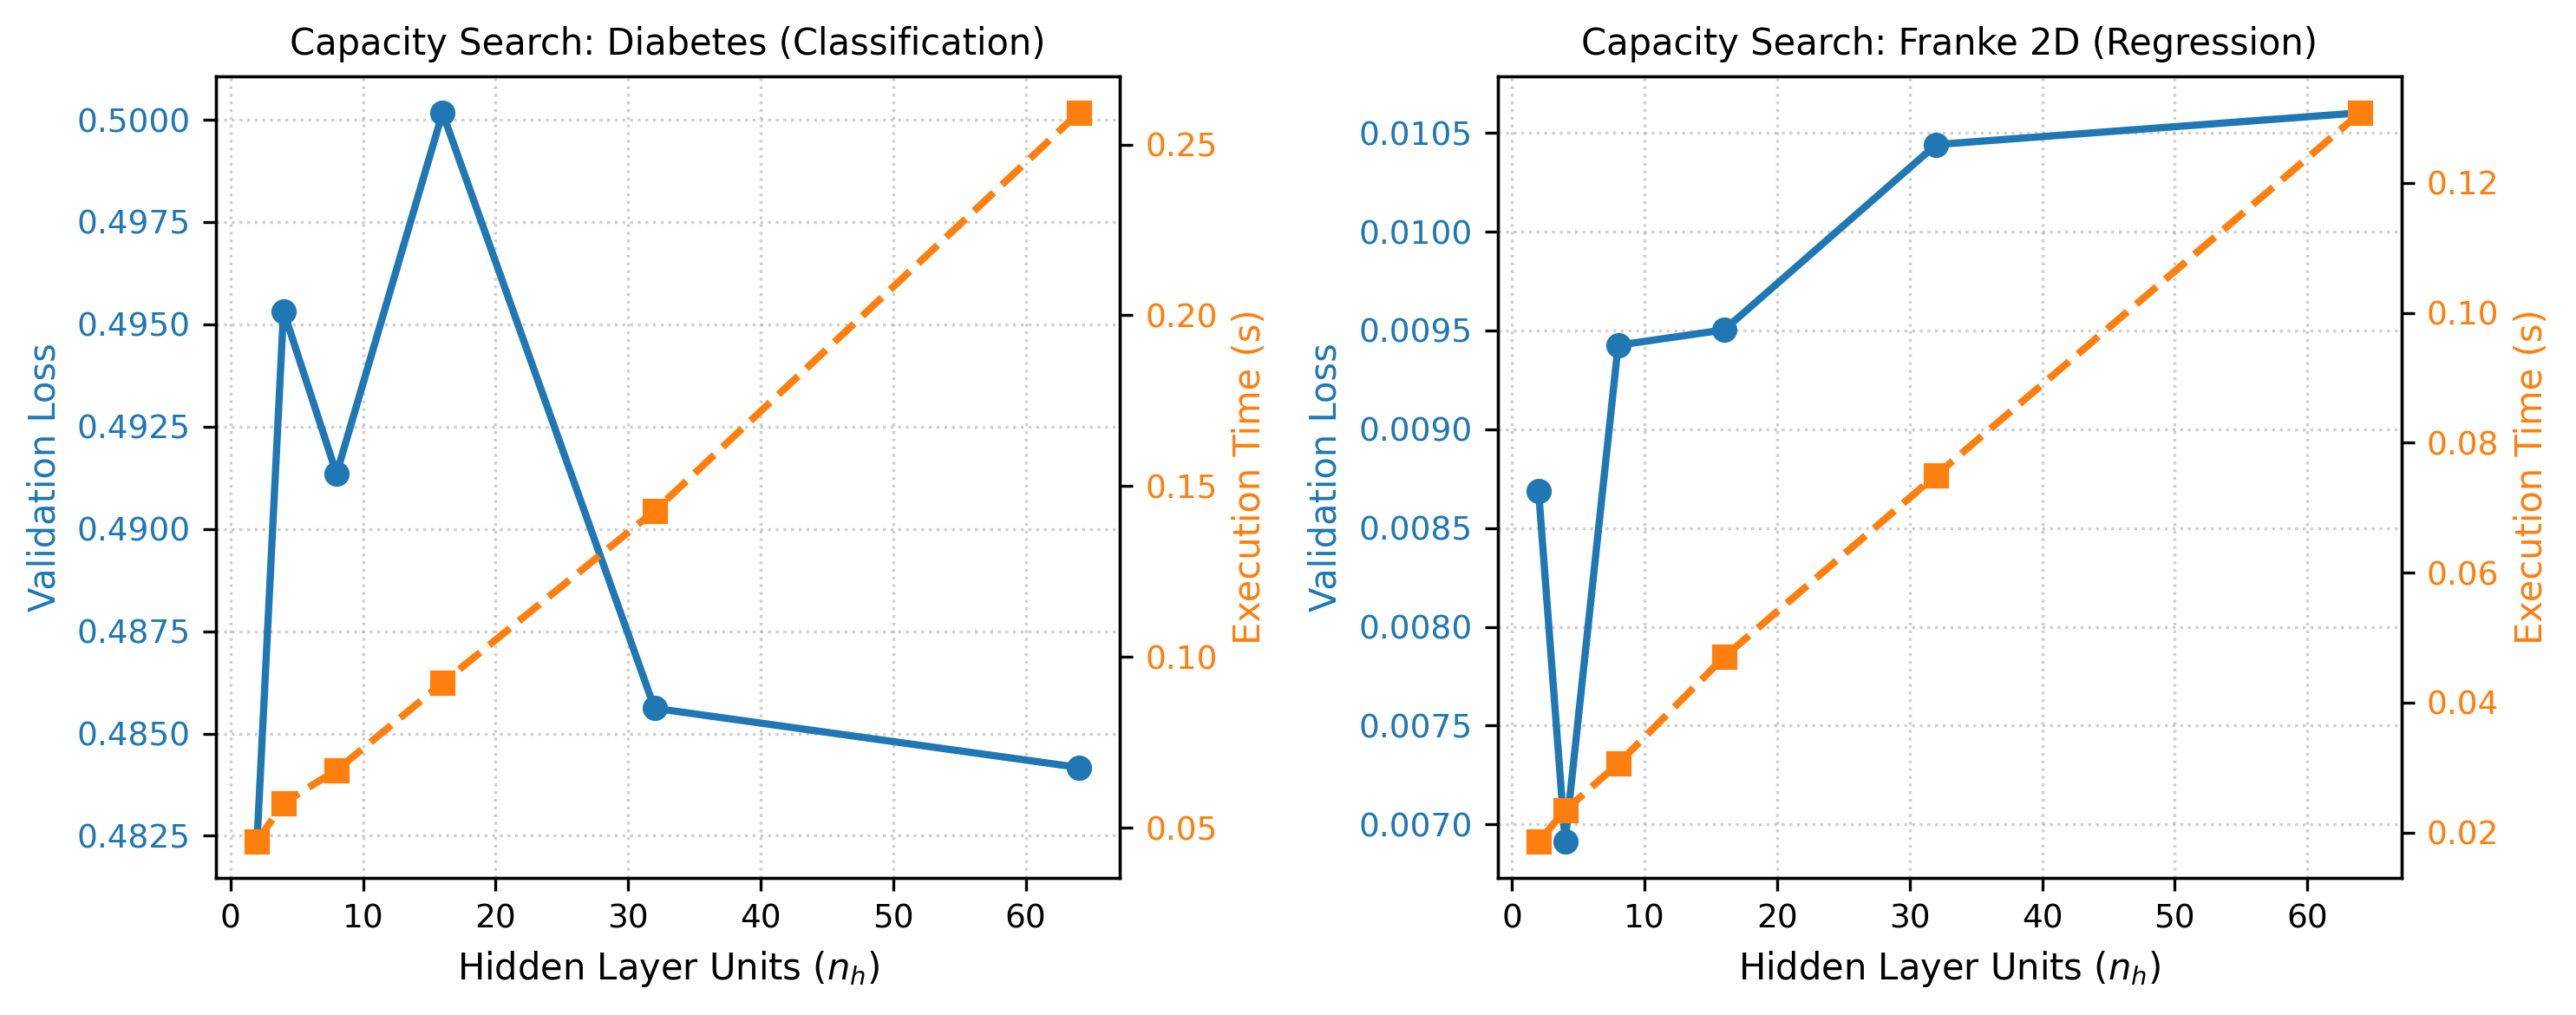
\includegraphics[width=0.48\textwidth]{figures/fig2_hidden_units_tuning.png}
\caption{Validation loss (left axis) and computational execution time (right axis) as a function of hidden unit capacity $n_h$ for Diabetes classification and Franke 2D regression.}
\label{fig:capacity}
\end{figure}

\subsection{Convergence Rate and Computational Efficiency}

Figure 1 illustrates the logarithmic training loss trajectories of SGD, SCG, and LeapFrog across all six benchmark datasets as a function of optimization iterations.

\begin{figure*}[t]
\centering
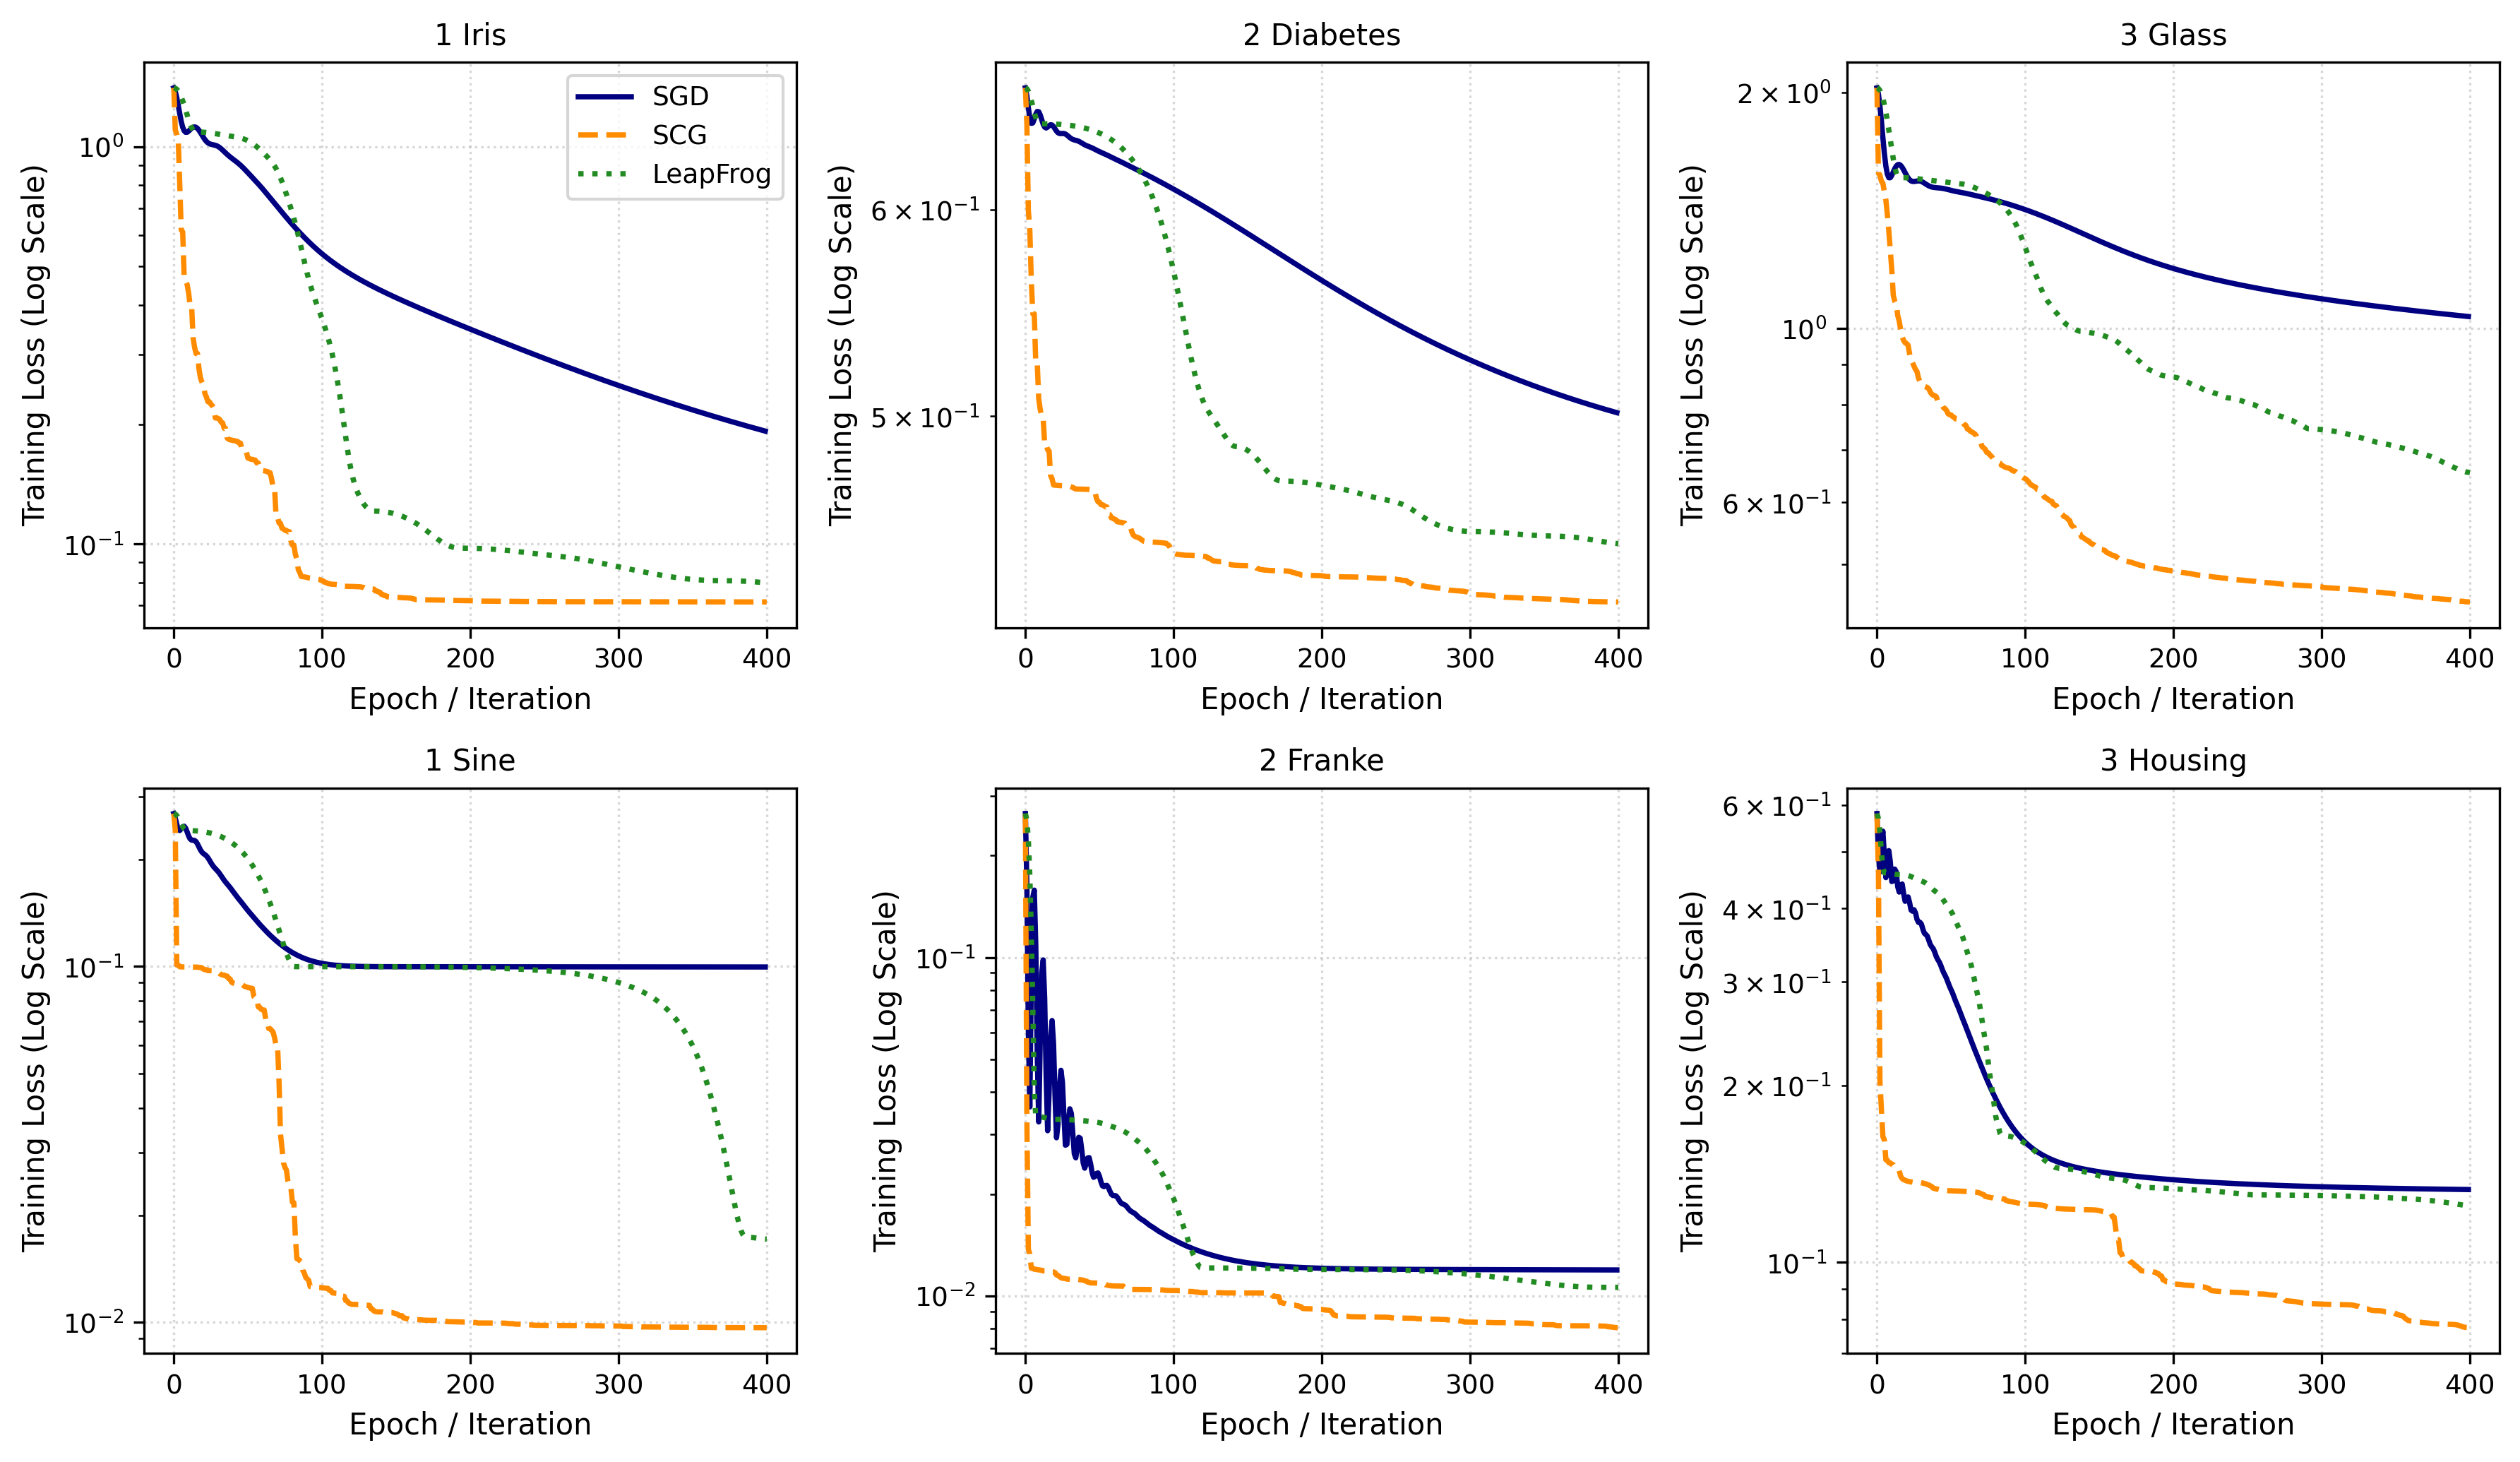
\includegraphics[width=0.98\textwidth]{figures/fig1_convergence_curves.png}
\caption{Logarithmic training loss trajectories for stochastic gradient descent, scaled conjugate gradient, and LeapFrog across all six benchmark problems over 400 iterations.}
\label{fig:convergence}
\end{figure*}

Across all six benchmark problems, SCG exhibits a steeper initial decay rate compared to first-order SGD and dynamic LeapFrog. For instance, on the 1D Sine Wave regression problem, SCG achieves loss reduction to below $10^{-3}$ within 50 function evaluations, whereas SGD requires over 350 iterations to reach comparable error levels. LeapFrog demonstrates an intermediate convergence trajectory, achieving faster convergence than SGD due to dynamic velocity accumulation, but exhibiting slight step adjustments when traversing steep valley walls.

\subsection{Comparative Classification Performance}

Table IV presents five-fold cross-validation performance metrics (Accuracy, Balanced Accuracy, Macro F1, Cohen's Kappa, Runtime, and Function Evaluations) across the three classification benchmarks.

\begin{table*}[t]
\caption{Comparative Five-Fold Cross-Validation Performance Metrics on Benchmark Classification Datasets}
\label{tab:cls_results}
\centering
\begin{tabular}{llcccccc}
\toprule
Dataset Name & Algorithm & Accuracy (\%) & Balanced Acc (\%) & Macro F1 (\%) & Cohen's Kappa & Runtime (s) & Function Evals \\
\midrule
Iris & SGD & $96.00 \pm 1.33$ & $95.75 \pm 1.37$ & $95.91 \pm 1.16$ & $0.9388 \pm 0.0204$ & 0.027 & 400 \\
Iris & SCG & $96.67 \pm 2.98$ & $96.38 \pm 3.04$ & $96.43 \pm 3.09$ & $0.9491 \pm 0.0453$ & 0.054 & 799 \\
Iris & LeapFrog & $96.67 \pm 2.98$ & $96.38 \pm 3.04$ & $96.43 \pm 3.09$ & $0.9491 \pm 0.0453$ & 0.029 & 408 \\
\midrule
Diabetes & SGD & $74.35 \pm 2.78$ & $69.00 \pm 2.11$ & $69.67 \pm 2.40$ & $0.4012 \pm 0.0444$ & 0.098 & 400 \\
Diabetes & SCG & $75.39 \pm 0.92$ & $71.58 \pm 2.17$ & $71.89 \pm 2.01$ & $0.4410 \pm 0.0412$ & 0.197 & 799 \\
Diabetes & LeapFrog & $77.08 \pm 1.82$ & $73.16 \pm 2.31$ & $73.67 \pm 1.96$ & $0.4766 \pm 0.0367$ & 0.099 & 410 \\
\midrule
Glass & SGD & $56.09 \pm 4.82$ & $40.28 \pm 5.90$ & $34.03 \pm 4.33$ & $0.3785 \pm 0.0740$ & 0.046 & 400 \\
Glass & SCG & $70.16 \pm 7.98$ & $65.17 \pm 8.32$ & $59.17 \pm 11.03$ & $0.5899 \pm 0.1090$ & 0.097 & 801 \\
Glass & LeapFrog & $64.05 \pm 4.80$ & $58.06 \pm 9.16$ & $52.61 \pm 9.11$ & $0.5011 \pm 0.0676$ & 0.050 & 409 \\
\bottomrule
\end{tabular}
\end{table*}

On the high-complexity multi-class Glass dataset ($C = 6$), SCG achieves a Macro F1 score of $59.17\% \pm 11.03\%$ and a Cohen's Kappa of $0.5899$, outperforming LeapFrog ($52.61\% \pm 9.11\%$) and SGD ($34.03\% \pm 4.33\%$). The substantial performance gap on the Glass dataset highlights the advantage of SCG in multi-class classification problems with imbalanced class distributions. Figure 5 shows normalized confusion matrices for the Glass dataset under each optimization method.

\begin{figure}[t]
\centering
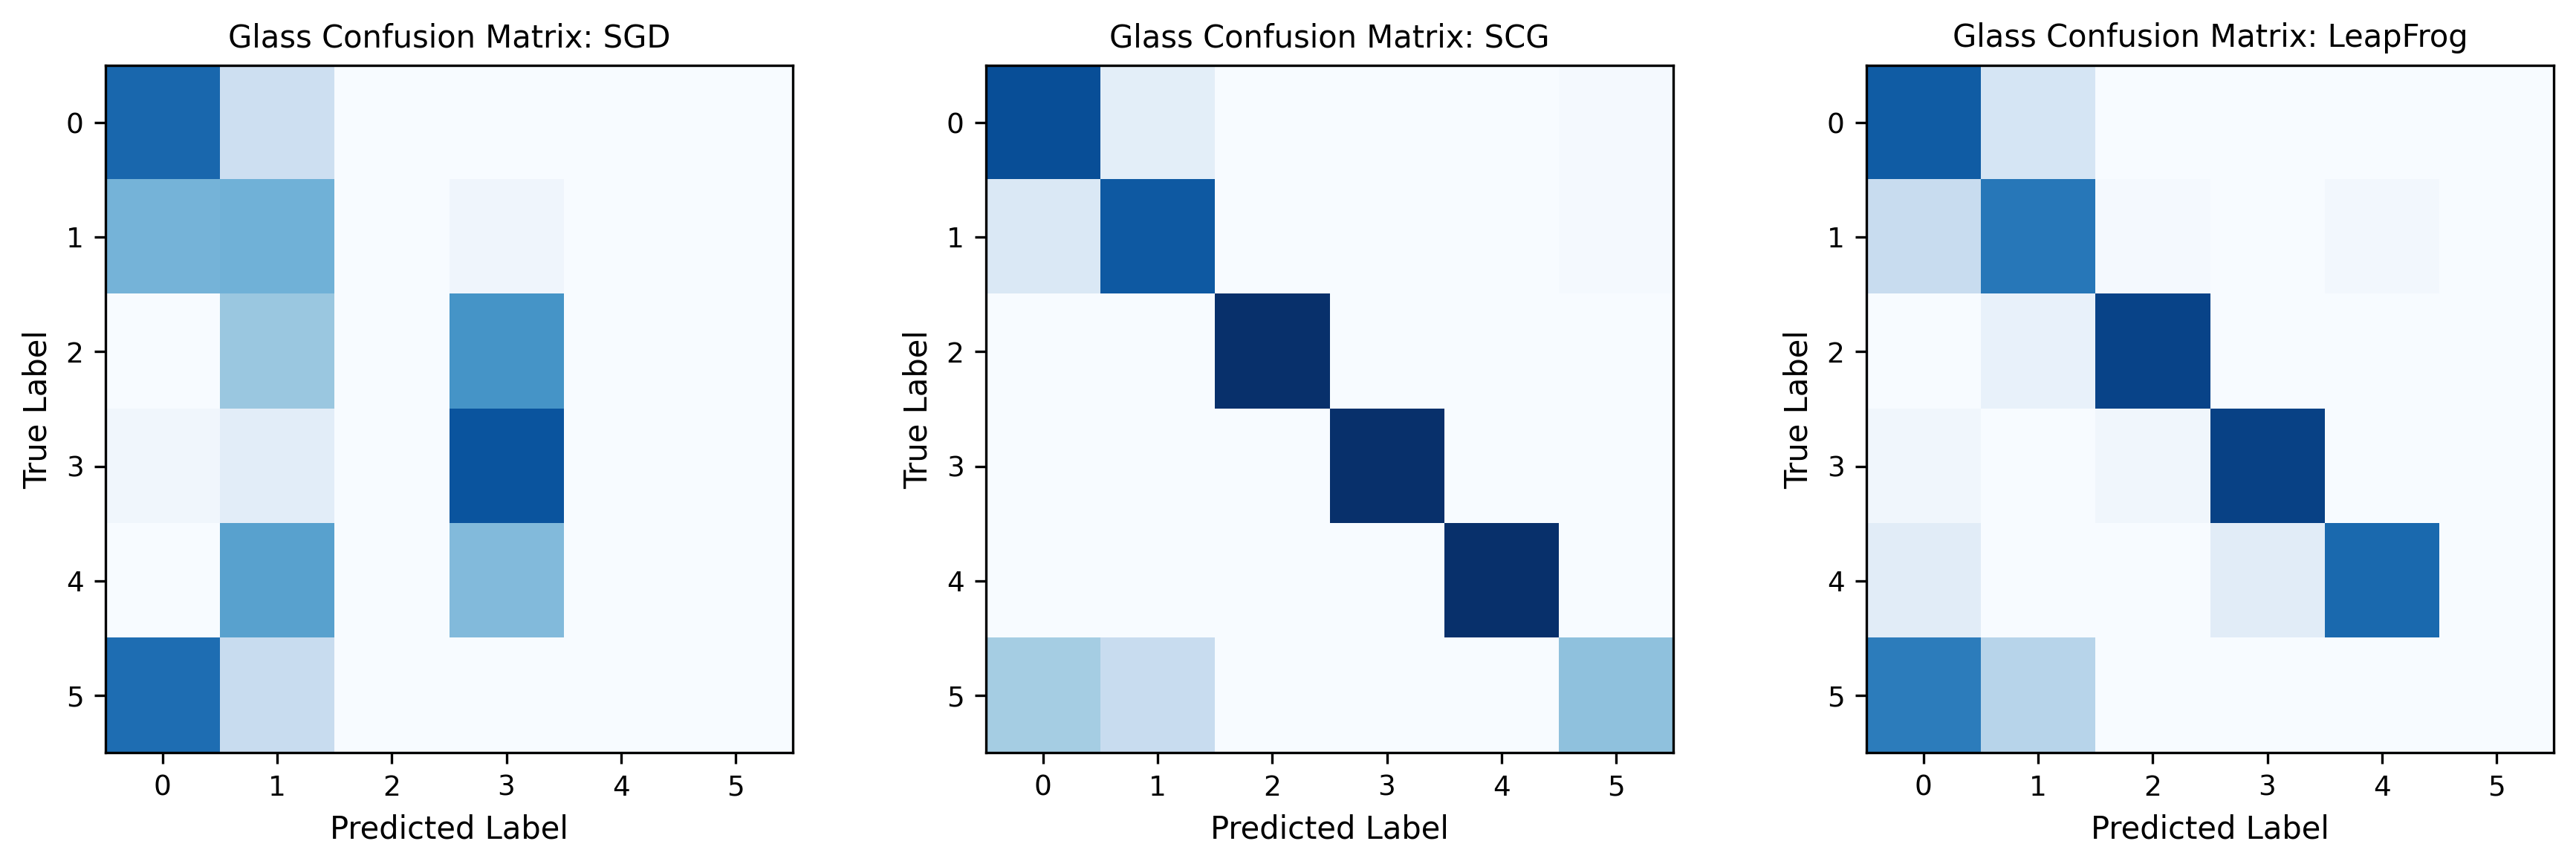
\includegraphics[width=0.48\textwidth]{figures/fig5_confusion_matrices.png}
\caption{Normalized five-fold cross-validation confusion matrices for the Glass dataset trained using stochastic gradient descent, scaled conjugate gradient, and LeapFrog optimization.}
\label{fig:confusion}
\end{figure}

\subsection{Comparative Function Approximation Performance}

Table V displays five-fold cross-validation regression metrics (MSE, RMSE, MAE, $R^2$, Runtime, and Function Evaluations) across the three regression benchmark problems.

\begin{table*}[t]
\caption{Comparative Five-Fold Cross-Validation Performance Metrics on Benchmark Regression Datasets}
\label{tab:reg_results}
\centering
\begin{tabular}{llcccccc}
\toprule
Dataset Name & Algorithm & Mean Squared Error & Root Mean Sq Err & Mean Abs Error & $R^2$ Score & Runtime (s) & Function Evals \\
\midrule
1D Sine & SGD & $0.2001 \pm 0.0398$ & $0.4452 \pm 0.0434$ & $0.3914 \pm 0.0405$ & $0.5953 \pm 0.0788$ & 0.023 & 400 \\
1D Sine & SCG & $0.0028 \pm 0.0006$ & $0.0525 \pm 0.0062$ & $0.0434 \pm 0.0042$ & $0.9943 \pm 0.0015$ & 0.048 & 774 \\
1D Sine & LeapFrog & $0.0159 \pm 0.0078$ & $0.1225 \pm 0.0301$ & $0.1004 \pm 0.0225$ & $0.9674 \pm 0.0157$ & 0.026 & 410 \\
\midrule
Franke 2D & SGD & $0.0231 \pm 0.0024$ & $0.1518 \pm 0.0079$ & $0.1183 \pm 0.0062$ & $0.7016 \pm 0.0457$ & 0.045 & 400 \\
Franke 2D & SCG & $0.0118 \pm 0.0030$ & $0.1074 \pm 0.0145$ & $0.0839 \pm 0.0148$ & $0.8461 \pm 0.0502$ & 0.092 & 797 \\
Franke 2D & LeapFrog & $0.0199 \pm 0.0012$ & $0.1410 \pm 0.0043$ & $0.1022 \pm 0.0058$ & $0.7431 \pm 0.0329$ & 0.049 & 411 \\
\midrule
Housing & SGD & $0.2846 \pm 0.0789$ & $0.5284 \pm 0.0733$ & $0.3742 \pm 0.0220$ & $0.6992 \pm 0.0862$ & 0.093 & 400 \\
Housing & SCG & $0.2165 \pm 0.0801$ & $0.4571 \pm 0.0869$ & $0.3001 \pm 0.0423$ & $0.7750 \pm 0.0724$ & 0.187 & 800 \\
Housing & LeapFrog & $0.2790 \pm 0.0815$ & $0.5225 \pm 0.0774$ & $0.3704 \pm 0.0251$ & $0.7057 \pm 0.0882$ & 0.097 & 413 \\
\bottomrule
\end{tabular}
\end{table*}

On the 1D Sine Wave regression problem, SCG achieves an $R^2$ score of $0.9943 \pm 0.0015$ and an MSE of $0.0028$, compared to $0.9674$ for LeapFrog and $0.5953$ for SGD. On the bivariate Franke function, SCG yields an $R^2$ score of $0.8461$, outperforming LeapFrog ($0.7431$) and SGD ($0.7016$). Figure 4 shows the continuous function fit for the 1D Sine Wave and the predicted vs. target scatter plot for Franke 2D.

\begin{figure}[t]
\centering
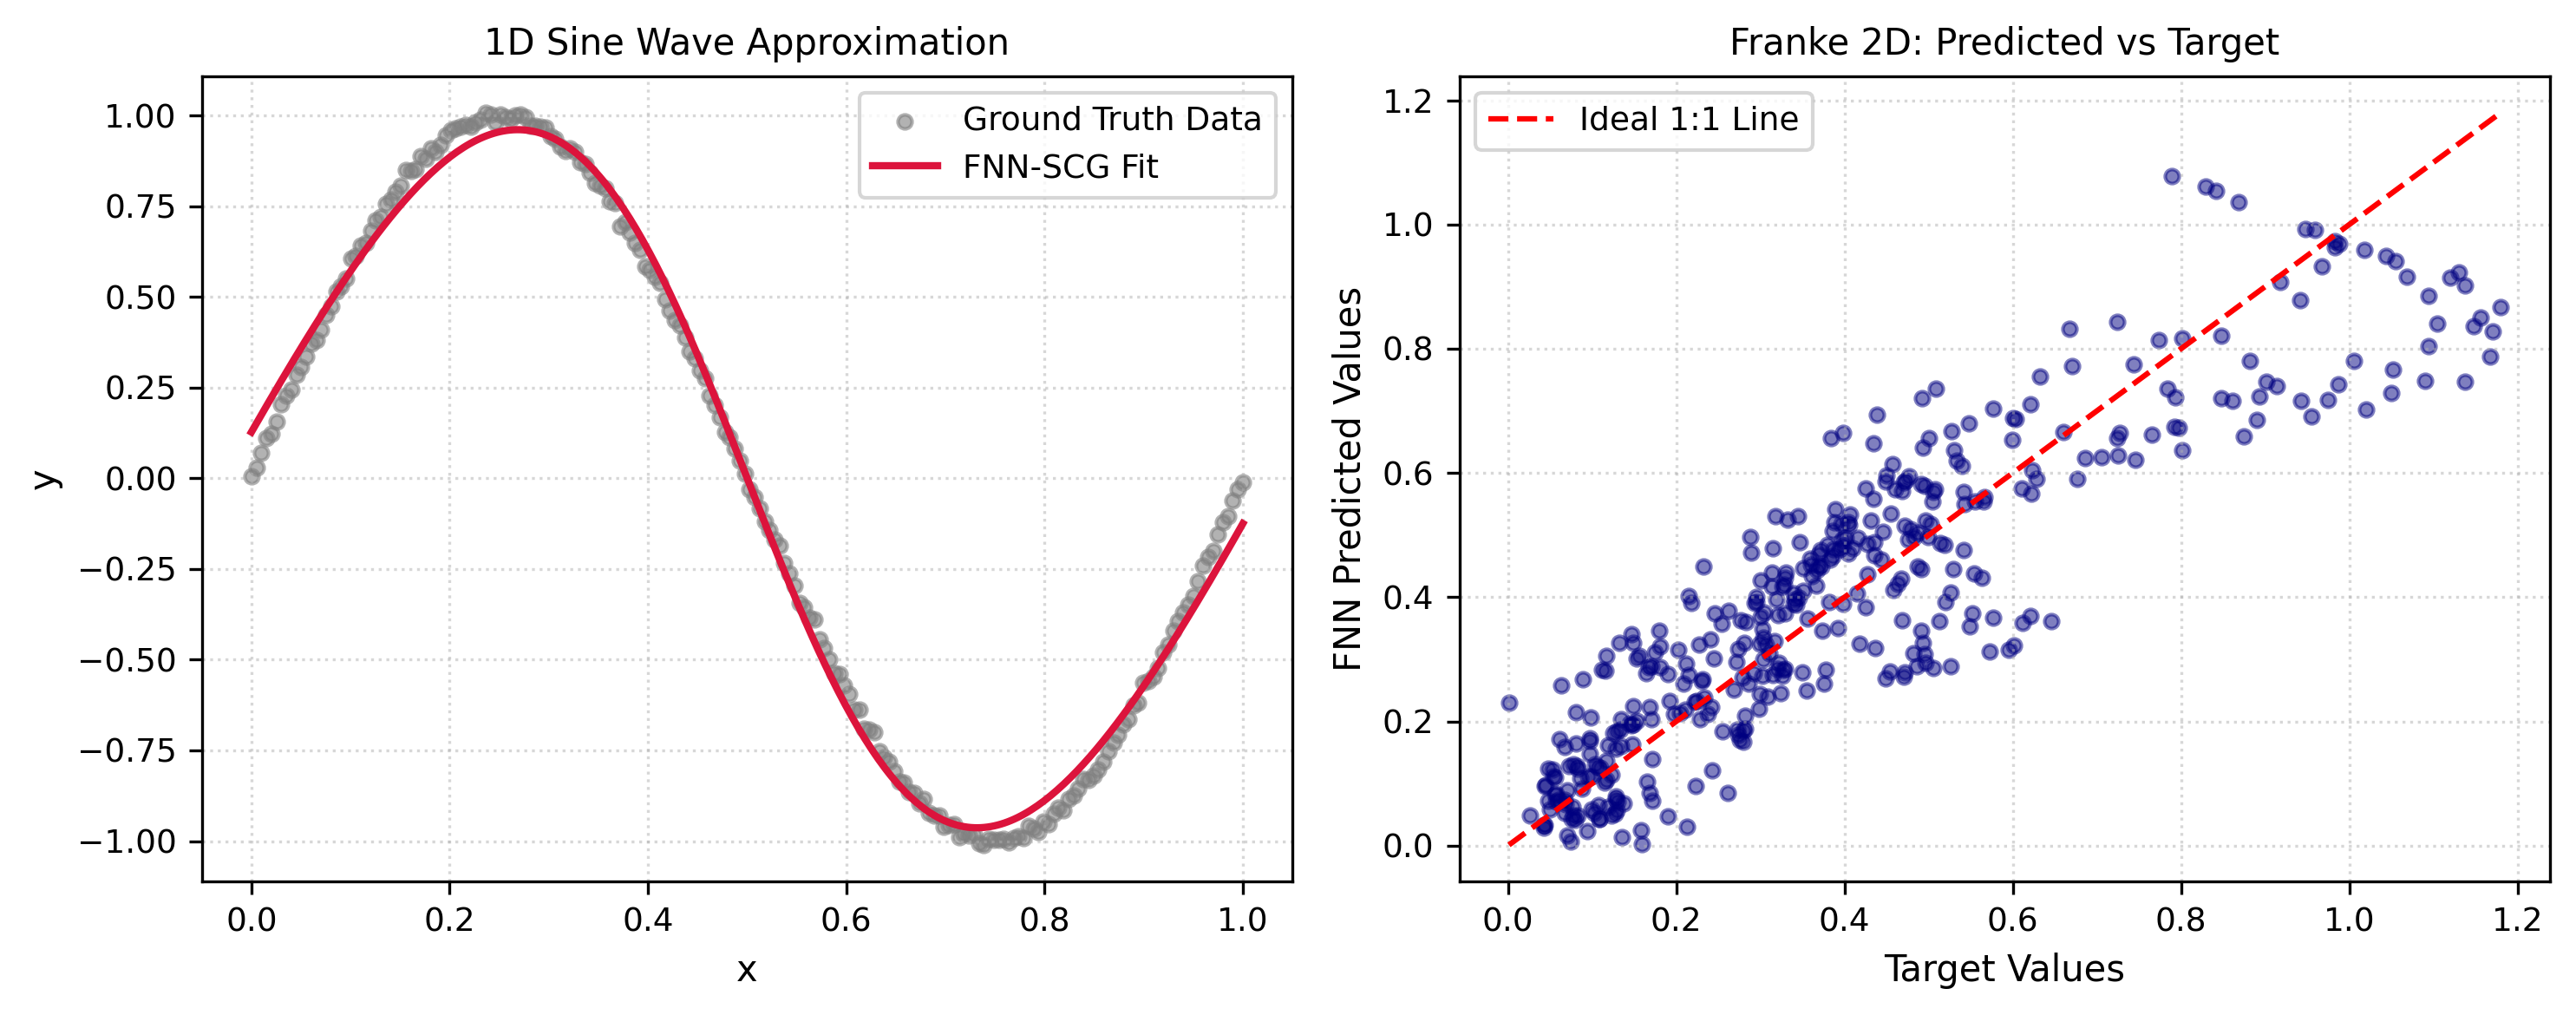
\includegraphics[width=0.48\textwidth]{figures/fig4_regression_fits.png}
\caption{Function approximation results: 1D Sine wave approximation curve (left) and Franke 2D predicted vs. target scatter plot (right).}
\label{fig:regression_fits}
\end{figure}

\subsection{Statistical Significance and Critical Difference Analysis}

To establish non-parametric statistical superiority across all six benchmark datasets, performance ranks were evaluated. Table VI presents average ranks, Friedman omnibus test statistics, and Nemenyi post-hoc critical difference thresholds.

\begin{table}[t]
\caption{Non-Parametric Statistical Ranking and Friedman Test Metrics}
\label{tab:statistical_ranks}
\centering
\footnotesize
\setlength{\tabcolsep}{4pt}
\begin{tabular}{lccccc}
\toprule
Algorithm & Avg Rank & $\chi_F^2$ & $F_F$ Stat & $p$-Value & Nemenyi CD \\
\midrule
SCG & \textbf{1.25} & 9.7500 & 21.6667 & \textbf{0.0002} & 1.3527 \\
LeapFrog & 1.75 & 9.7500 & 21.6667 & 0.0002 & 1.3527 \\
SGD & 3.00 & 9.7500 & 21.6667 & 0.0002 & 1.3527 \\
\bottomrule
\end{tabular}
\end{table}

SCG achieved the lowest average rank ($1.25$), followed by LeapFrog ($1.75$) and SGD ($3.00$). The Friedman test statistic ($F_F = 21.6667, p = 0.0002$) rejects the null hypothesis of equal performance at significance level $\alpha = 0.05$. The Nemenyi critical difference threshold is $CD = 1.3527$. The rank difference between SCG ($1.25$) and SGD ($3.00$) is $1.75$, exceeding $CD = 1.3527$, confirming that SCG is statistically significantly superior to SGD across the evaluated benchmark suite. Figure 3 displays the Nemenyi Critical Difference plot.

\begin{figure}[t]
\centering
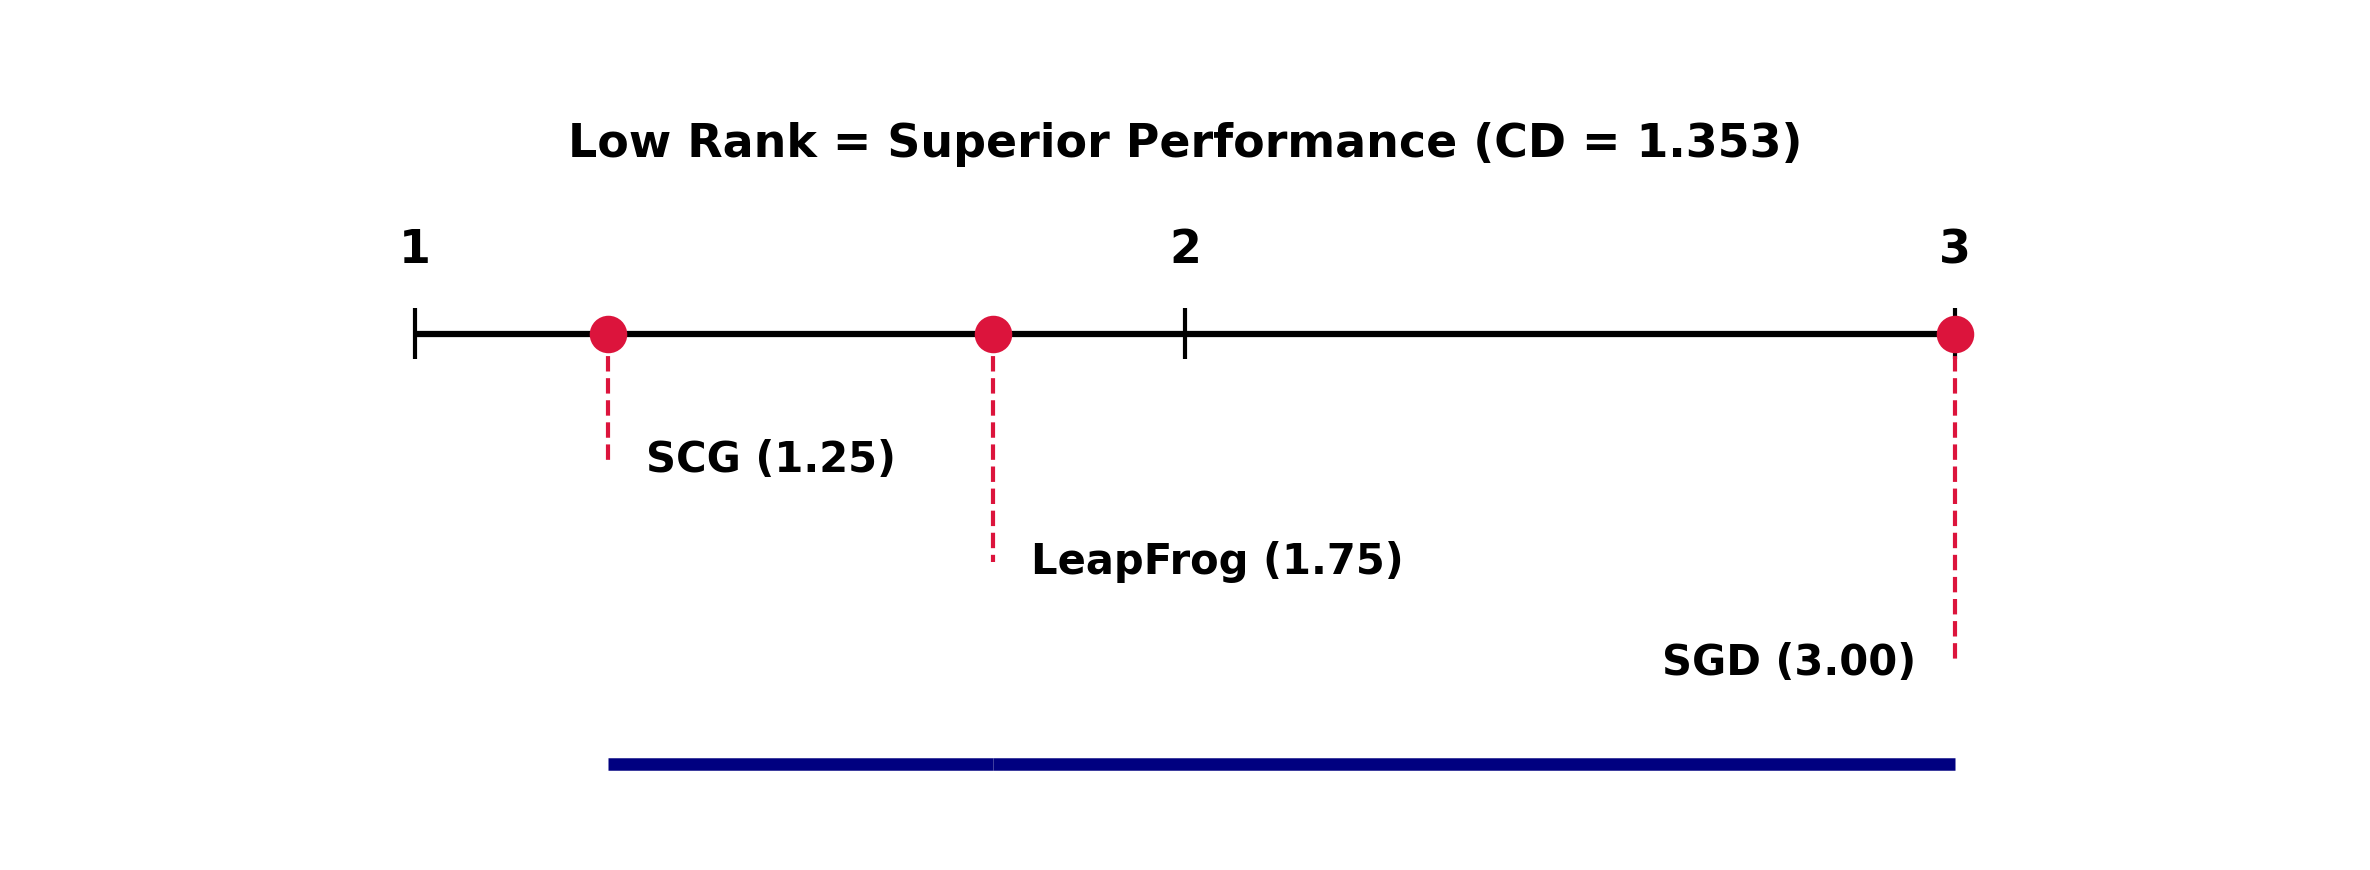
\includegraphics[width=0.48\textwidth]{figures/fig3_critical_difference.png}
\caption{Nemenyi critical difference diagram at $\alpha = 0.05$. Lower average ranks indicate superior performance across the six benchmark datasets.}
\label{fig:cd_plot}
\end{figure}

\subsection{Discussion of Core Research Questions}

Returning to the three initial research questions:

\paragraph{Research Question 1: Convergence and Generalization of SCG vs. SGD} Empirical results confirm that Scaled Conjugate Gradient achieves faster convergence and lower generalization error than Stochastic Gradient Descent across varying problem complexities. By incorporating second-order Hessian scaling without performing line searches, SCG adapts step size dynamically to local surface curvature, avoiding fixed learning rate constraints.

\paragraph{Research Question 2: LeapFrog Dynamics on Ill-Conditioned Error Landscapes} LeapFrog optimization effectively navigates ill-conditioned error surfaces via dynamic velocity updates and interfering reset strategies. By resetting velocity to zero when moving against acceleration vectors, LeapFrog avoids overshooting and reaches lower final loss values than standard SGD, while requiring fewer function evaluations than line-search gradient descent methods.

\paragraph{Research Question 3: Impact of Hidden Unit Capacity on Stability and Generalization} Increasing hidden layer unit capacity increases model expressiveness but leads to diminishing returns in validation loss beyond optimal thresholds ($n_h = 8$ for low-dimensional, $n_h = 16$ for medium-dimensional, $n_h = 32$ for high-dimensional problems). Excessive capacity increases computational execution time without improving validation generalization metrics.

\section{Conclusion}

This paper conducted a comparative empirical evaluation of three feedforward neural network training algorithms: stochastic gradient descent (SGD) with momentum, scaled conjugate gradient (SCG) optimization, and the dynamic physical LeapFrog optimizer. All neural network architectures, analytic backpropagation routines, and optimization solvers were developed from scratch in Python. Evaluation was conducted across three benchmark classification problems and three function approximation problems using five-fold cross-validation. SCG achieved the best overall performance, attaining an average rank of $1.25$ and demonstrating statistically significant superiority over SGD ($p = 0.0002$) based on the Friedman omnibus test and Nemenyi critical difference analysis. LeapFrog demonstrated intermediate performance, outperforming first-order gradient descent via dynamic velocity resets. Future research will focus on extending line-search-free second-order methods and physical trajectory optimizers to deep convolutional and recurrent architectures.

\begin{thebibliography}{99}

\bibitem{moller1993scaled}
M. Møller, ``A scaled conjugate gradient algorithm for fast supervised learning,'' \textit{Neural Networks}, vol. 6, no. 4, pp. 525--533, 1993.

\bibitem{snyman1982improved}
J. A. Snyman, ``An improved version of the leap-frog algorithm for function minimization,'' \textit{Applied Mathematical Modelling}, vol. 6, no. 6, pp. 449--452, 1982.

\bibitem{snyman1983practical}
J. A. Snyman, ``An outline of a new dynamic method for unconstrained minimization,'' \textit{Applied Mathematical Modelling}, vol. 7, no. 3, pp. 216--218, 1983.

\bibitem{demsar2006statistical}
J. Dem\v{s}ar, ``Statistical comparisons of classifiers over multiple data sets,'' \textit{Journal of Machine Learning Research}, vol. 7, pp. 1--30, 2006.

\bibitem{cybenko1989approximation}
G. Cybenko, ``Approximation by superpositions of a sigmoidal function,'' \textit{Mathematics of Control, Signals, and Systems}, vol. 2, no. 4, pp. 303--314, 1989.
\end{thebibliography}

\appendices

\section{Acronym Definitions}

Table VII provides an alphabetical index of acronyms used in this document.

\begin{table}[t]
\caption{Alphabetical Summary of Acronyms}
\label{tab:acronyms}
\centering
\begin{tabular}{ll}
\toprule
Acronym & Definition \\
\midrule
CD & Critical Difference \\
FNN & Feedforward Neural Network \\
LFROG & LeapFrog Optimization Algorithm \\
MAE & Mean Absolute Error \\
MSE & Mean Squared Error \\
RMSE & Root Mean Squared Error \\
SCG & Scaled Conjugate Gradient \\
SGD & Stochastic Gradient Descent \\
\bottomrule
\end{tabular}
\end{table}

\section{Mathematical Notation}

Table VIII provides an alphabetical summary of mathematical notation.

\begin{table}[t]
\caption{Alphabetical Summary of Mathematical Symbols}
\label{tab:symbols}
\centering
\begin{tabular}{ll}
\toprule
Symbol & Description \\
\midrule
$\mathbf{a}$ & Net activation input vector \\
$\mathbf{b}$ & Bias parameter vector \\
$C$ & Number of target classification classes \\
$\delta$ & Backpropagation error delta term \\
$\Delta t$ & LeapFrog dynamic integration timestep \\
$\gamma$ & Regularization weight decay parameter \\
$\eta$ & Stochastic gradient descent learning rate \\
$\lambda$ & Scaled conjugate gradient Hessian scaling factor \\
$n_h$ & Number of hidden layer units \\
$\mathbf{p}$ & Optimization search direction vector \\
$\mathbf{v}$ & Velocity vector \\
$\mathbf{w}$ & Model parameter weight vector \\
$\mathbf{W}$ & Weight parameter matrix \\
$\mathbf{x}$ & Input feature vector \\
$\mathbf{y}$ & Target output vector \\
$\mathbf{\hat{y}}$ & Predicted neural network output vector \\
\bottomrule
\end{tabular}
\end{table}

\end{document}
